\chapter{Literature Review}\label{ch:litreview}
\section{An Introduction to LID and DID systems}
Dialect identification (DID) is a specialised task of Language Identification (LID)
which identifies the dialects within a language. It poses more challenges compared to LID, 
as dialects share many acoustic, linguistic features and speaker characteristics. An accurate LID 
or DID allows for more specialised models to be used for other speech related tasks including ASR, speech transcription and 
Natural Learning Processing (NLP).
Over time the methodology of LID and DID systems has evolved. 
Traditionally Phonemic Modelling was used to construct Arabic DIDs which is discussed further in Section
\ref{sec:phonematic}. Then traditional machine learning networks were used, which is explored in Section 
\ref{sec:tradML}. Current research is exploring the viability of utilising transfer based learning methods 
for LIDs and DIDs, which is detailed in Section \ref{sec:transfer}. Table \ref{tab:MLapplications} compares 
the accuracies that were achieved both with traditional machine learning methods and transfer learning. The two Arabic DIDs in the table will be discussed 
further in this section, and it can be seen 
that transfer learning using a wav2vec pretrained model has only been tested for LID which was fairly successful with an accuracy of 95.5\%


\begin{table}[hbt!]
    \begin{center}
    \begin{tabular}{|m{3cm} | m{2.5cm} | m{2cm} |  m{3cm} |  m{1.7cm} | m{2cm} |}
        \hline
        \textbf{Application} & \textbf{Features} & \textbf{Pretrained Model} & \textbf{Downstream Model} &\textbf{Accuracy} &\textbf{Year, Paper}\\
        \hline
        Arabic DID \newline(17 dialects) & 80 dimensional Fbank & 
        Transformer Based Network (trained on ADI17) & CNN & 86.29\% & (2020), \cite{lin_transformer-based_2020} \\
        \hline
        Arabic DID \newline(5 dialects) & i-vector + FBANK + \newline word + \newline char + \newline phoneme & 
        N/A & E2E CNN+RNN+FC, DNN+SNN (feature extraction) & 81.36\% & (2018), \cite{shon_convolutional_2018} \\
        \hline
        LID (English, Spanish, French, German, Russian, and Italian) & Spectrograms & 
        Resnet50 & CNN + RESnets & 89\% & (2019), \cite{salameh_fine-grained_2018}\\
        \hline
        LID (Arabic, English, Malay, French, Spanish, German, Persian, and Urdu) & 
        Acoustic features (MFCC + GMM + i-vector) & N/A & ESA-ELM (Enhanced Self- Adjusting Extreme Learning Machine) 
        & 96.25\% & (2018), \cite{tjandra_improved_2021}\\
        \hline
        LID \newline(26 languages) & N/A & wav2vec 2.0 & pooling layer + linear layer & 95.5\% & (2021), \cite{mohamed_arabic_2021}\\
        \hline
    \end{tabular}
    \caption{Recent Machine Learning Implementations of LIDs \& DIDs.}
    \label{tab:MLapplications}
    \end{center}
\end{table}

\pagebreak
\section{Traditional Methodologies}
\subsection{Phonematic Modelling}\label{sec:phonematic}
A phoneme in linguistics is the smallest unit of sound which can convey meaning (for instance, the sound /c/ in cat). 
Phonematic modelling utilises recognisers to identify the phonemes present within an audio segment. 
Different dialects usually have different phoneme combinations and so, the identified phonemes are mapped 
to identify a dialect. In the paper \cite{biadsy_dialect_2011} this technique was used to construct an Arabic DID for 4 dialects (Gulf, Iraqi, Levantine, and Egyptian) plus MSA which took advantage of  
English, Arabic, Japanese phone recognisers to identify the phoneme differences between the dialects as seen in Figure \ref{fig:phoneRec}. This method was able to achieve high accuracy 
levels for identifying MSA with F-Measures above 98\% and the highest of the dialects was Egyptian Arabic with an F-Measure of 90.2\% with 30s test-utterances. As seen in Figure \ref{fig:phoneAcc},  
phonemic modelling for Arabic struggled when given shorter utterances and had particularly low accuracies for the Gulf dialect. The key challenges with using phoneme modelling is that 
it relies on the distinguishing phonemes to be present in the test data and for finer regional dialects it requires there to be more shared phonemes between the dialects.

\begin{figure}[H]
    \CommonHeightRow{%
        \begin{floatrow}[2]%
            \ffigbox[\FBwidth]
            {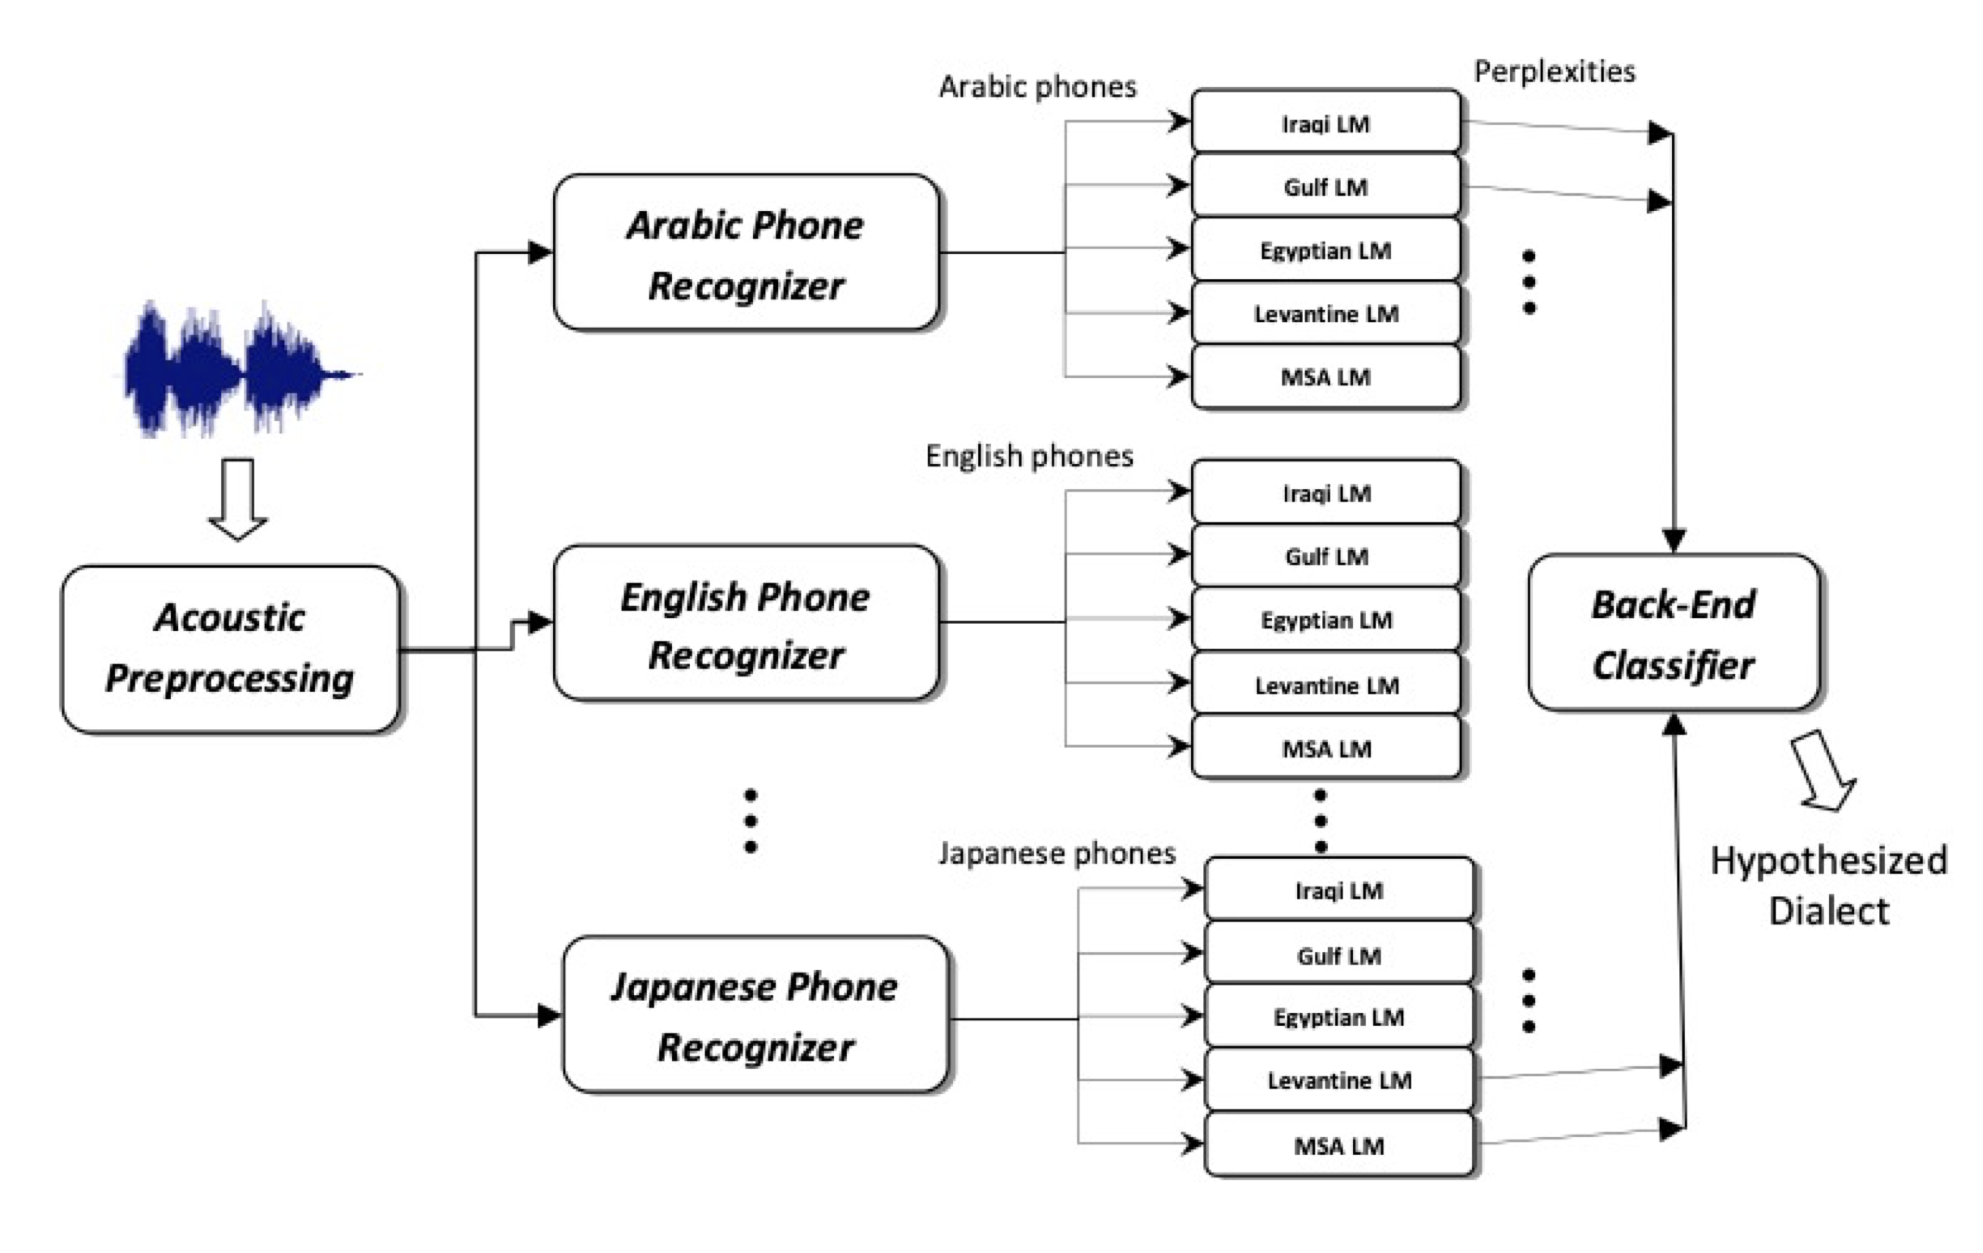
\includegraphics[height=6cm]{phonemModeling.png}}
            {\caption{Parallel Phone Recognition \newline Followed by Language Modeling (PRLM)\newline for Arabic DID \cite{biadsy_spoken_2009}.}}\label{fig:phoneRec}
            \ffigbox[\FBwidth]
            {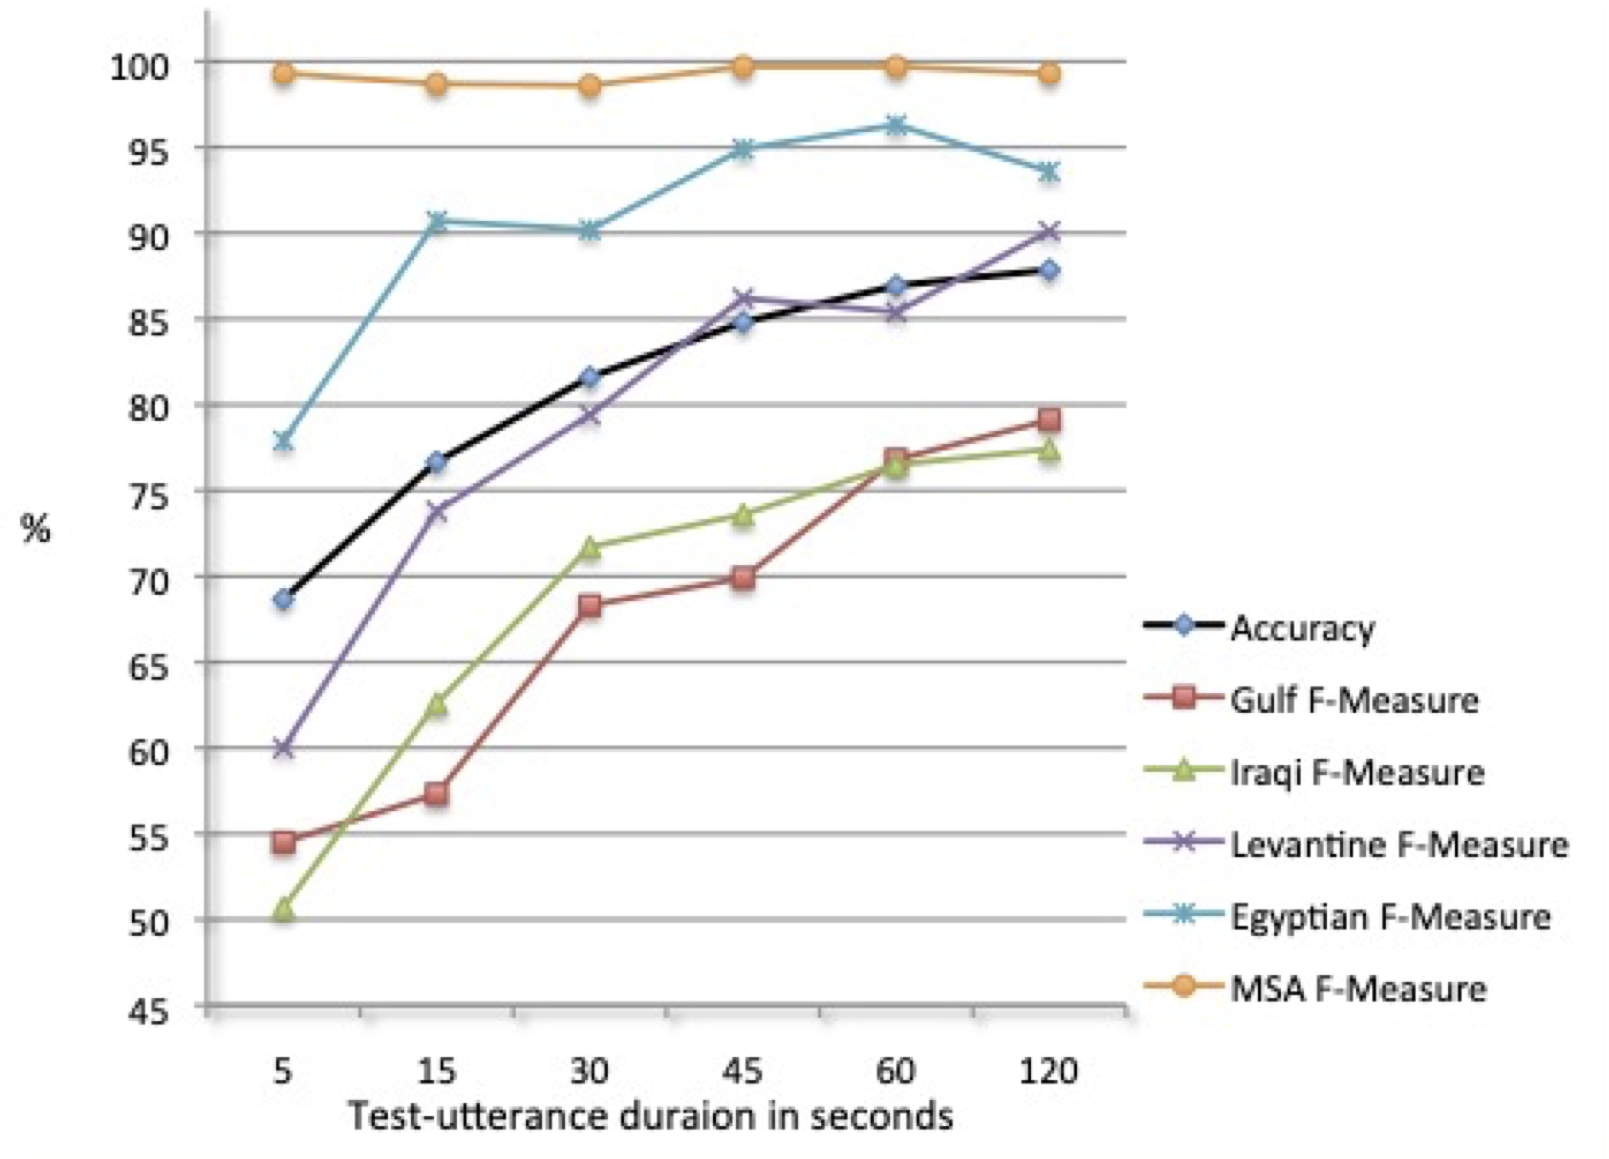
\includegraphics[height=6cm]{accuraciesPhonemModeling.png}}
            {\caption{The accuracies and F-Measures \newline of the five-way classification task with different test-utterance durations \cite{biadsy_spoken_2009}.}}\label{fig:phoneAcc}
        \end{floatrow}}%
\end{figure}

\subsection{Traditional Machine Learning}\label{sec:tradML}
Traditional Machine learning has been used for both LID and DID systems as explored in papers \cite{albadr_spoken_2018,lin_transformer-based_2020,miao_lstm-tdnn_2019,miao_new_2019,revay_multiclass_2019,shon_convolutional_2018,tjandra_improved_2021}. 
They operate by extracting key features from the training audio, which could be acoustic and/or linguistic, then using some form 
of traditional machine learning structure to learn the differences between dialects based on the extracted features. Implemented in the papers \cite{lin_transformer-based_2020,miao_lstm-tdnn_2019,miao_new_2019,shon_convolutional_2018}
are ransformer based networks which are constructed with a similar structure to that shown in Figure \ref{fig:transformerLID}. Simple transformer 
networks were compared to networks which used a combination of CNN, LSTM networks along with the transformer network. Convolutional Neural Networks (CNN)
are composed of three types of layers, a convolutional layer, pooling layer and a fully-connected (FC) layer, with a greater amount of layers the complexity of 
the network increases. CNNs learn through using filters to detect certain features in the training data and adjusting its weights accordingly. The Arabic DID explored in paper \cite{liu_roberta_2019}
used the ADI17 dataset which will be used in this thesis was able to achieve the highest accuracy of 86.29\% when cascaded with a CNN network.  
In contrast, Bidirectional Long Short Term Memory (BiLSTM) is created from two Recurrent Neural Networks (RNN). It has the ability to combine information from both past and future inputs. 
The structure of BiLSTM is shown in Figure \ref{fig:BiLTSM}. 
Although, there are no papers showing the effectiveness of using BiLSTMs specifically for Arabic DID, LSTMs were used in \cite{miao_lstm-tdnn_2019,miao_new_2019}, transformer based networks 
and were able to achieve an accuracy of well over 90\% for all the ADI17 dialects in \cite{miao_new_2019}. As well as this, the papers \cite{samih_neural_2017,zaidan_arabic_2014} explored the use of BiLSTMs in text based Arabic DIDs and paper \cite{tseng_mandarin-english_2021} explored
its use in Mandarin/English LID with XLS-R producing a 92.7\% accuracy.

\begin{figure}[h!]
    \centering
    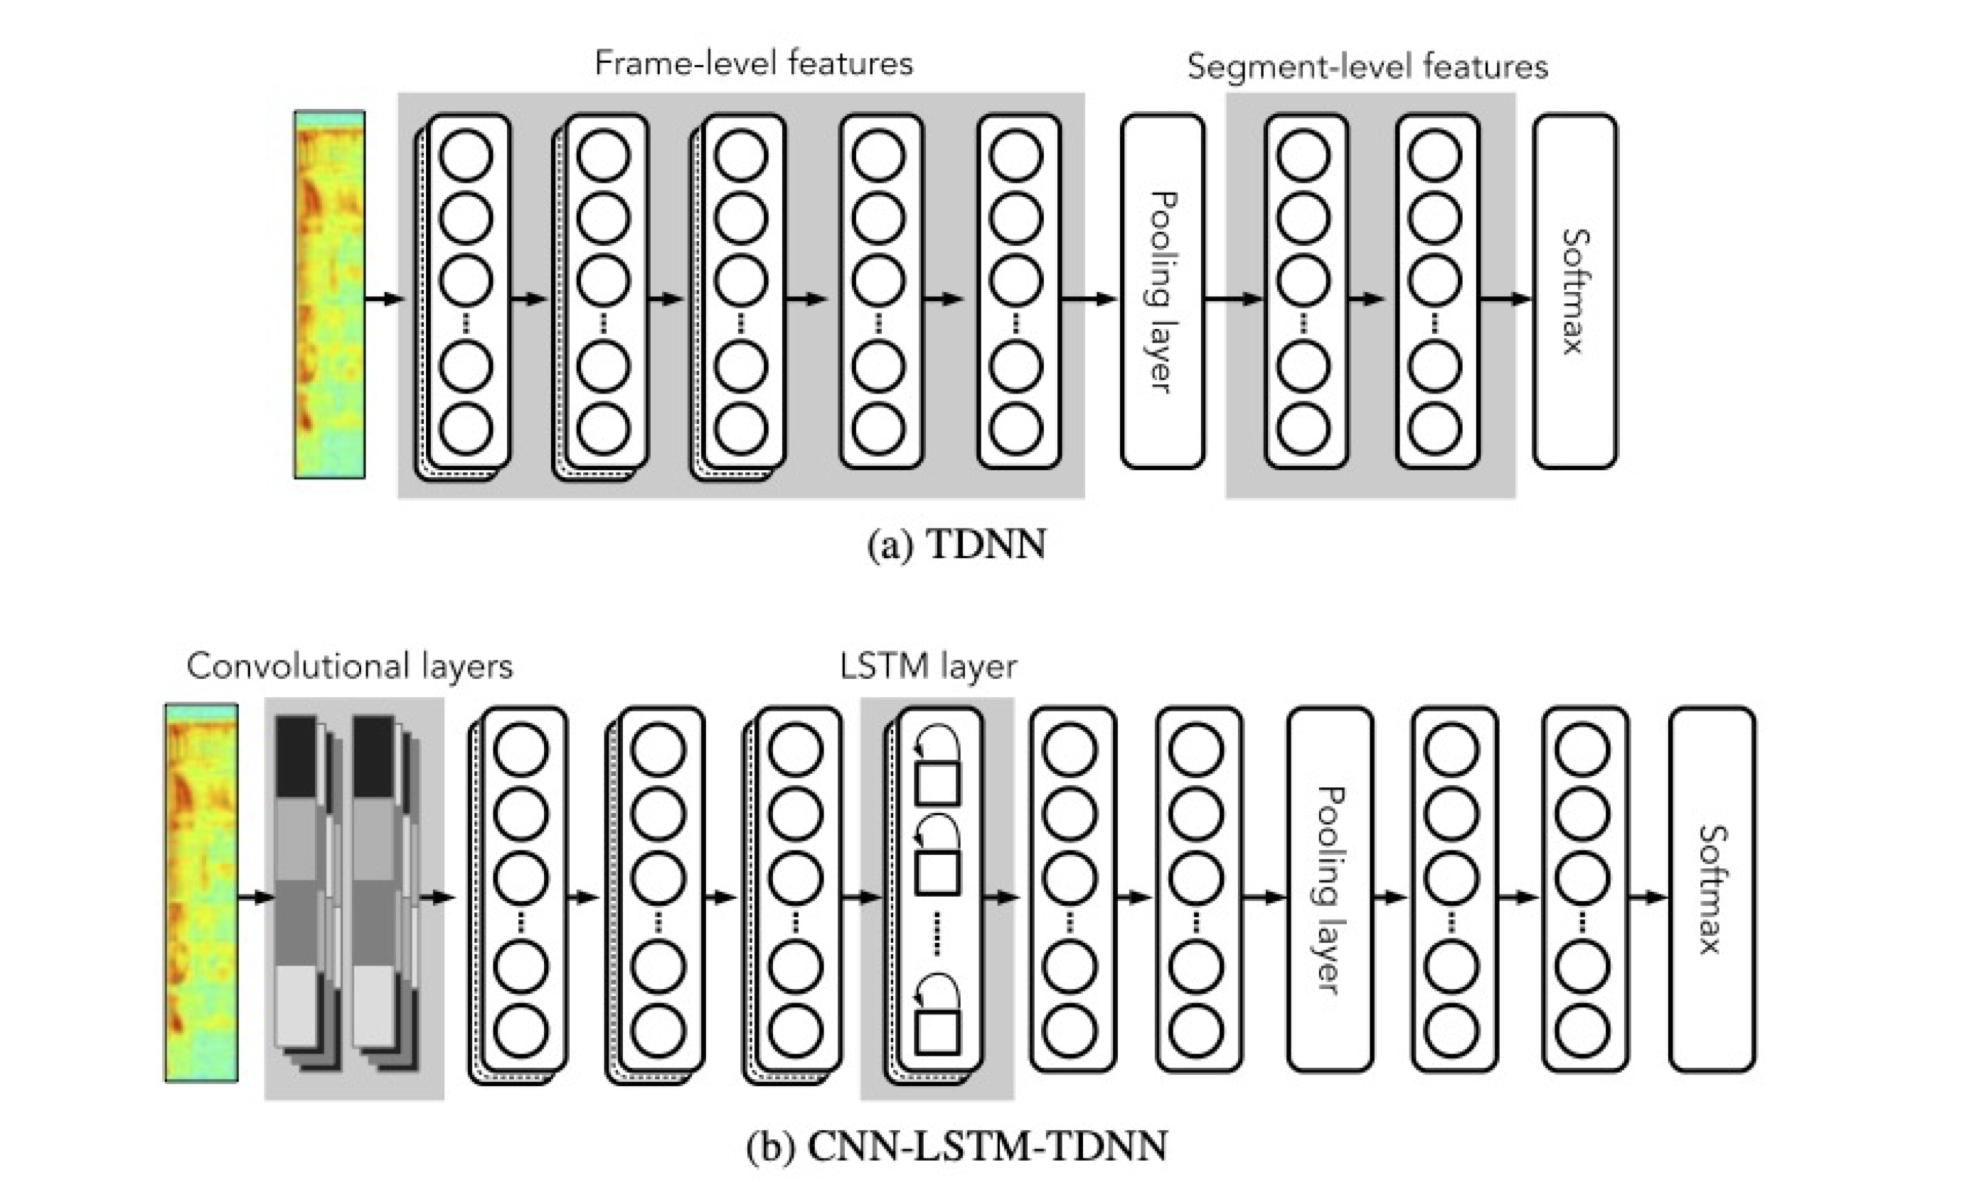
\includegraphics[width=\textwidth]{TransformerNetwork.png}
    \caption{Transformer Network based LID \cite{miao_new_2019}.}
    \label{fig:transformerLID}
\end{figure}

\begin{figure}[h!]
    \centering
    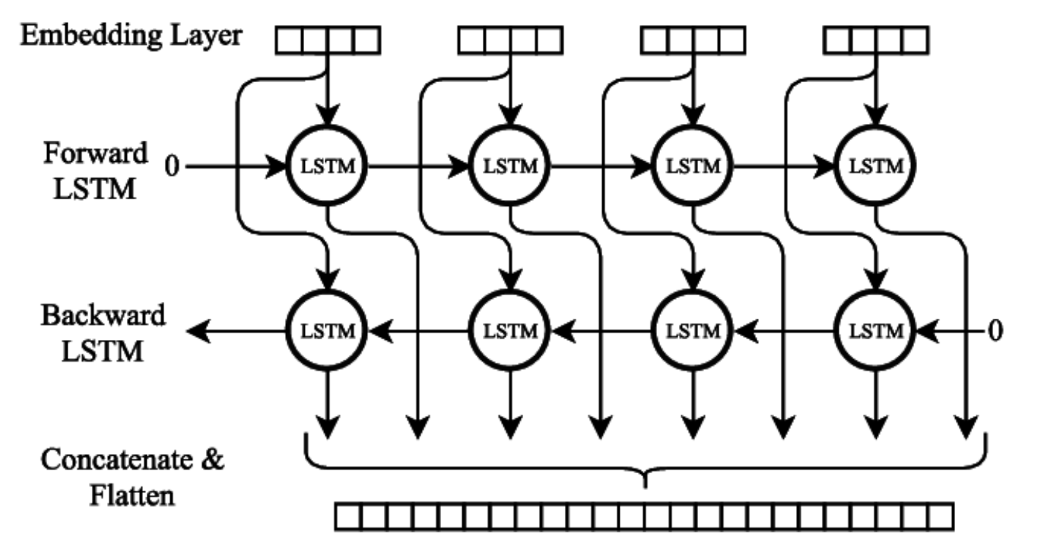
\includegraphics[width=\textwidth]{BiLTSM.png}
    \caption{BiLTSM Structure \cite{cornegruta_modelling_2016}.}
    \label{fig:BiLTSM}
\end{figure}


\section{Transfer Learning}\label{sec:transfer}
Transfer learning is a form of deep machine learning which focuses on adapting a pretrained model to execute a 
similar task. The pretraining enables rapid learning for modelling the task and often requires less data to 
achieve a high level of accuracy in the secondary class. For the task of LID and DID, this often means applying 
a pretrained model designed for speech tasks like ASR, speech synthesis etc. Transfer learning is a relatively new method for optimising 
machine learning to complete a task and so, there are not a vast amount of papers exploring its use for some more niche tasks 
like LID and DID. Papers \cite{hussein_arabic_2021, habash_guidelines_2008, mohamed_arabic_2021, wang_fine-tuned_2021} have shown significant increases in accuracy using pretrained models for tasks 
such as emotion recognition, ASR and NLP. 

In addition to a pretrained model, a transfer learning system often has a downstream model connected to it that allows the model to 
adapt to more specific tasks. The system can then be trained end to end (E2E) or fine-tuned in portions, tuning the pretrained model, then 
the downstream. It was found in the paper \cite{wang_fine-tuned_2021}, which explored E2E training for wav2vec and HuBERT for the tasks Speaker Verification (SV), Intent Classification (IC) and Slot Filling (SF), that on average using E2E training 
provides more accurate systems. For example, looking at their results for wav2vec, E2E outperformed segmented training by 12.47\% in SER, decreased EER by 3.26\% in SV, improved accuracy in IC by 39.98\% and SF by 36.66\%. 
Thereby, this thesis will employ E2E training for the system. 

\subsection{Pretrained Models}\label{sec:pretrain}
The pretrained models are semi-self supervised machine learning models often designed by large tech companies, then trained on large amounts of 
unlabeled and small amounts of labelled data. There are several pretrained models available for use for speech processing the main ones that will be explored are HuBERT, wav2vec 2.0 and XLSR developed by Facebook. 
Wav2vec 2.0 is designed for speech data, consisting of a feature encoder, context network, quantisation module and 
a contrastive loss layer. 
Wav2vec is pretrained using a contrastive task, masking a unit in the feature vector then predicting what 
should be in that unit. In the case where the prediction is wrong a negative score is given and when right a positive, and the network then adjusts its weights accordingly.  
HuBert is a hidden unit bidirectional and shares a structure with wav2vec 2.0 using a transformer based networks and contrastive based learning, although it uses BERT. 
BERT is able to process a segment of speech simultaneously learning the surrounding context of a word. It aimed to improve wav2vec through the use of BERT prediction loss and 
was able to produce up to 19\% and 13\% relative WER reduction for a 1B parameter model. XLS-R is a fine-tuned variant of wav2vec 2.0, that is trained using data from 128 different languages collected from  BABEL, MLS, CommonVoice and VoxPopuli speech corpa. 
Tuning the model on languages other than English reduced error rates 14-34\% relative on average \cite{babu_xls-r_2021}. It has also shown to operate 
with a higher degree of accuracy on low resource languages compared to other models as shown in Figure \ref{fig:XLSRBLEU}. 
The paper \cite{mohamed_arabic_2021} compared the accuracy when using no pretrained model, wav2vec 2.0 and XSL-R on a 26 language LID. The highest accuracy was consistently achieved by XLS-R as seen in 
Figure \ref{fig:XLSRLID}, the highest being 95.7\% with 100hrs of labelled training data. 
Hence, this thesis will be using XLS-R and benchmarking it against wav2vec 2.0, HuBERT will not be tested as 
for the scope of this thesis it is too ambitious to explore more than two pretrained models. 

There hasn't been any research into the application of pretrained models for Arabic DIDs but there has been limited research into using wav2vec for LID systems. 
The papers \cite{babu_xls-r_2021,mohamed_arabic_2021,tjandra_improved_2021} demonstrate it as a possible methodology for LID. The paper \cite{mohamed_arabic_2021} was able to achieve an accuracy of 95.5\% for their 26 language LID, utilising only 
a simple pooling layer and linear layer as their downstream model as shown in Figure \ref{fig:wav2vec}. So, fine-tuning of the last two layers of wav2vec 2.0 will be the base method explored in this thesis. 

\begin{figure}[h!]
    \centering
    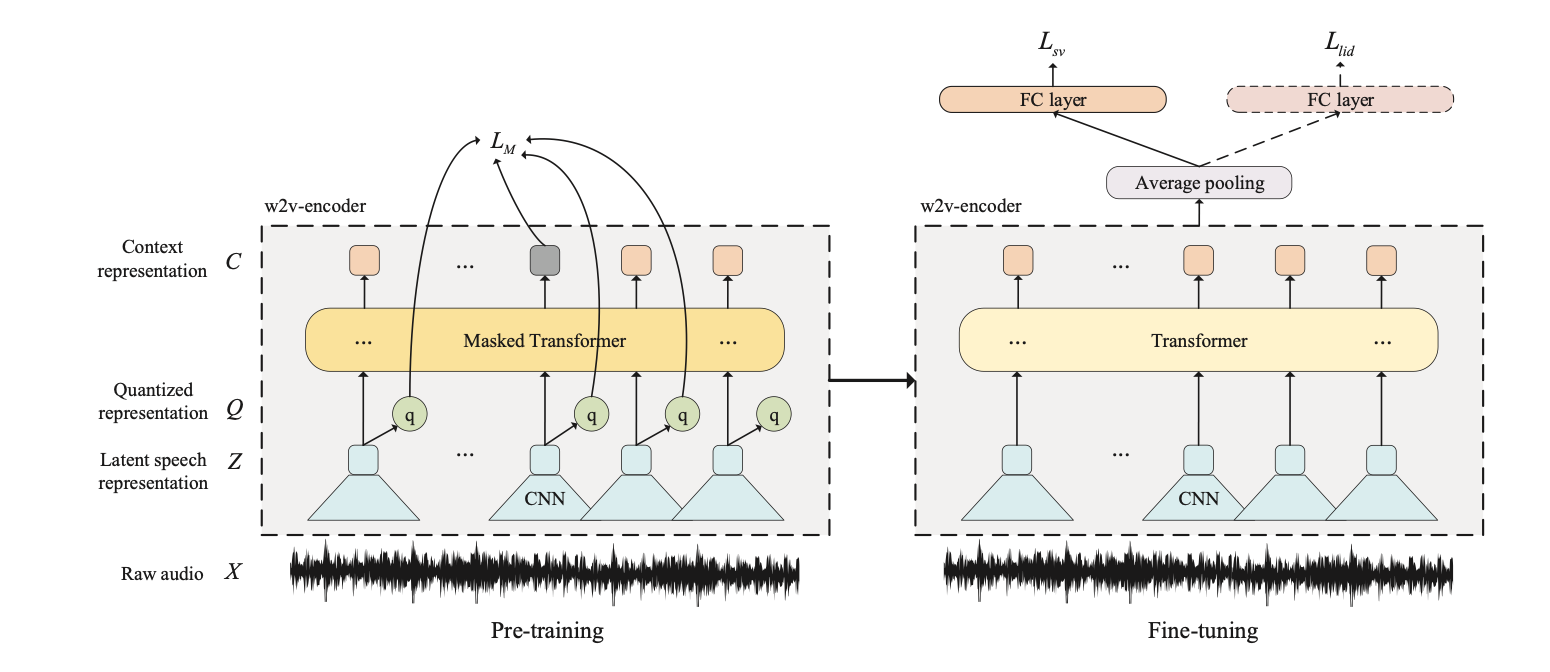
\includegraphics[width=\textwidth]{wav2vecLID.png}
    \caption{wav2vec 2.0 LID \cite{mohamed_arabic_2021}.}
    \label{fig:wav2vec}
\end{figure}

\begin{figure}[H]
    \CommonHeightRow{%
        \begin{floatrow}[2]%
            \ffigbox[\FBwidth]
            {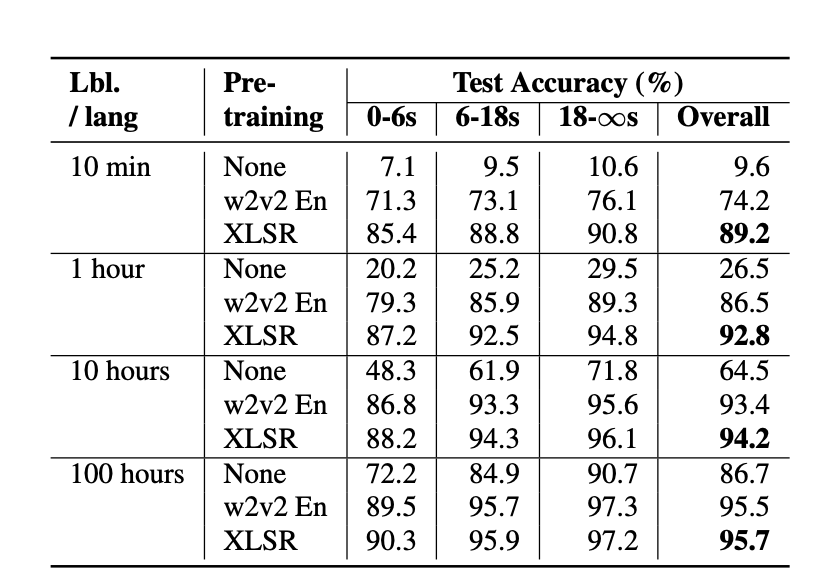
\includegraphics[height=6cm]{XLS-R-acc.png}}
            {\caption{26 language LID test accuracy \cite{mohamed_arabic_2021}.}}\label{fig:XLSRLID}
            \ffigbox[\FBwidth]
            {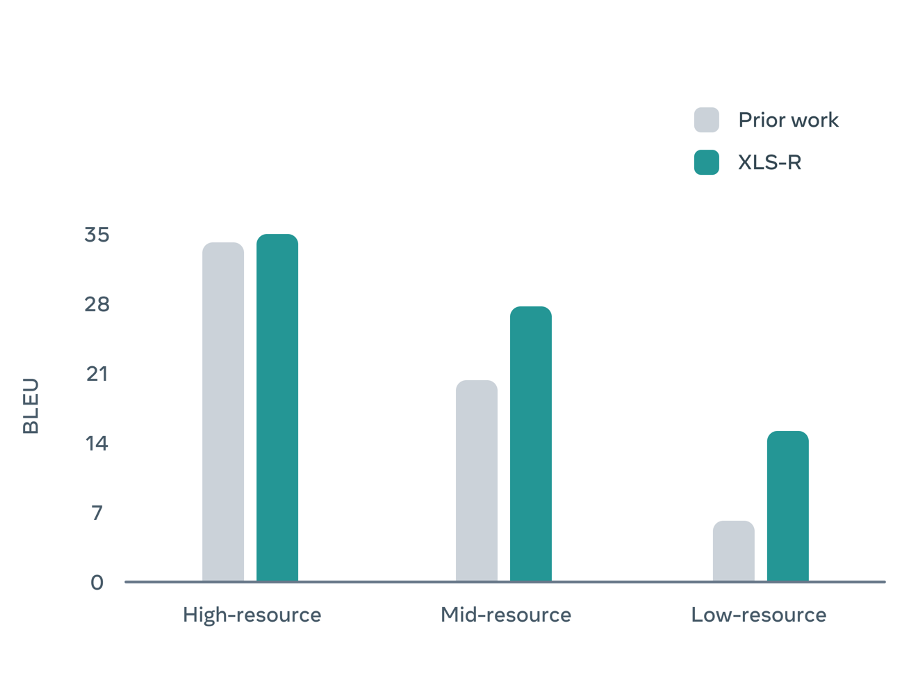
\includegraphics[height=7cm]{XLS-R.png}}
            {\caption{XLS-R BLEU Accuracy when Translating to English \cite{noauthor_xls-r_nodate}}}\label{fig:XLSRBLEU}
        \end{floatrow}}%
\end{figure}
